\chapter{Решение} \label{chapt3}

\section{Получение данных} \label{sect3_1}
Для решения задачи классификации нейронной сетью требуется наличие данных для обучения. Датасетов с настоящей проблемой в открытом доступе не нашлось, поэтому данные пришлось получать вручную. За основу был взят датасет OpenImageDataset[2] - набор изображений на более чем тысячу разных классов. Из него был взят подкласс Dog, в котором было 20000 изображений собак. Далее эти данные были размечены на Яндекс.Толоке. Каждое изображение было показано пользователю Толоки с вопросом “В какой позиции собака находится на этом фото”. Фотографии были размечены с пятикратным перекрытием, т.е. каждое изображение размечалось пять раз разными людьми.
На выходе получился скромного размера датасет, часть изображений в нём не подходили под постановку задач, но на выходе имелась следующая информация:
\begin{enumerate}
    \item Поза собаки (стоит, сидит, лежит на спине, лежит на боку)
    \item Поза хвоста собаки (вверх, вниз, прямо)
    \item Рот собаки (открыт, закрыт, высунут язык)
    \item Уши собаки (торчат, опущены)
    \item Количество собак в кадре
    \item Загорожена ли собака в кадре
    \item Ограничивающая рамка (bounding box) вокруг собаки.
    \item Ограничивающая рамка ушей, хвоста и рта собаки.
\end{enumerate}

\section{Проверка задачи на решаемость} \label{sect3_2}
После сбора данных, была предпринята попытка обучить нейронную сеть классифицировать полученные изображения. В лоб эта задача решается тяжело, из-за низкого качества входных данных и изначально малой обучающей выборки. Поэтому пришлось работать с обучающей выборкой. Были предприняты следующие меры для улучшения работы системы.
\begin{itemize}
    \item Все изображения были обрезаны по ограничивающей рамке собаки. И это дало сильный прирост в качестве классификации, 55\% -> 65\% на 5 классах
    \item Дополнительно были размечены изображения, где собака видна плохо, и были удалены из выборки. Это сократило размер и без того маленькой выборки, не сильно улучшив данные, т.к. качество разметки на Толоке достаточно низкое.
    \item Добавлены аугментации обучающей выборки. Аугментации позволяют нейронной сети не запоминать обучающие данные точь-в-точь, что снижает её способность к переобучению. Добавило около 2\% точности, 65-67\%
    \item Проведена очистка изображений. Из обучающей выборки были исключены изображения с несколькими собаками и собаками, которых не видно целиком. Это дало ощутимый прирост, но обучающая выборка сократилась до недопустимо маленьких размеров. Добавлено около 3\% точности, 67\%->69\%
    \item Использование transfer learning (переносимость обучения) - все модели что использовались здесь не обучались заново. Они обучались на ResNet34 уже предобученной классифицировать 1000 классов ImageNet(другого открытого датасета с изображениями).

\end{itemize}
\section{Эксперименты} \label{sect3_3}

\subsection{Создание нового датасета} \label{subsect3_3_1}
Учитывая прошлые ошибки было принято решение собрать датасет заново, используя опыт, полученный при разметке первого.

Главные изменения заключаются в следующем:
\begin{enumerate}
    \item Датасет собирается итеративно по небольшим частям и выводы делаются сразу
    \item Размер каждого класса удерживается на одинаковом уровне
    \item Проводится учёт всех изображений, которые тяжело размечать.
\end{enumerate}{}

\subsection{Первые 300 изображений} \label{subsect3_3_2}
Были собраны изображения собак по 100 изображений на целевой класс. На них была обучена простейшая архитектура, т.н. ShallowNet с одним свёрточным слоем.
Результаты следующие:
\begin{itemize}
    \item При классификации «в лоб» достигается точность в 60\%
    \item При обрезании изображений по ограничительной рамке собаки, точность увеличивается до 68\%
    \item При использовании черно-белых изображений точность также возрастает до 68\%
\end{itemize}

Где нейронная сеть ошибается:

В статье Amy Bearman и Cathering Dong \cite{Bearman2015HumanPE} указывается что нейронным сетям тяжело распознать позу, при наличии окклюзий, поворотов и переворотов, сильных перспективных искажений, и множественных объектов.

\begin{figure}[ht] 
  \center
  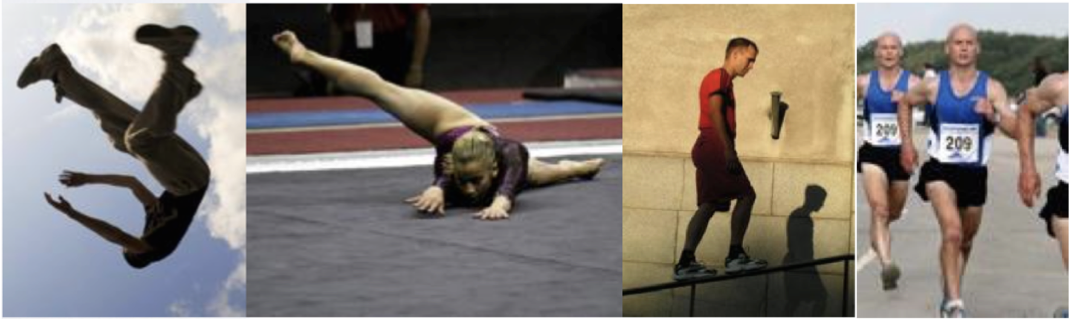
\includegraphics [scale=0.5] {hazards}
  \caption{Позы, которые трудно определить: повороты, перспектиные искажения, окклюзии и множественные объекты} 
  \label{img:hazards}  
\end{figure}

